\documentclass{article}

\usepackage[paperwidth=7.4in,paperheight=3.9in,margin=0in]{geometry}
\usepackage{tikz}
\usetikzlibrary{arrows.meta,positioning}
\usepackage[T1]{fontenc}
\usepackage{helvet}
\renewcommand{\familydefault}{\sfdefault}
\pagestyle{empty}

\definecolor{ink}{HTML}{0F172A}
\definecolor{muted}{HTML}{475569}
\definecolor{line}{HTML}{CBD5E1}
\definecolor{soft}{HTML}{F8FAFC}
\definecolor{blue}{HTML}{2563EB}
\definecolor{green}{HTML}{16A34A}
\definecolor{amber}{HTML}{D97706}
\definecolor{rose}{HTML}{E11D48}
\definecolor{violet}{HTML}{7C3AED}
\definecolor{cyan}{HTML}{0E7490}

\tikzset{
  card/.style={rounded corners=3pt, draw=line, line width=0.45pt, fill=soft},
  box/.style={rounded corners=2pt, align=center, draw=line, line width=0.38pt,
    fill=white, inner sep=2.0pt, text=ink, font=\fontsize{4.9}{5.4}\selectfont},
  context/.style={box, fill=cyan!9, draw=cyan!55, minimum width=0.75in, minimum height=0.24in},
  dag/.style={box, fill=violet!8, draw=violet!45, minimum width=0.72in, minimum height=0.22in},
  outcomeSmall/.style={box, fill=violet!8, draw=violet!45, minimum width=0.48in, minimum height=0.18in,
    font=\fontsize{4.2}{4.6}\selectfont},
  arch/.style={box, fill=blue!8, draw=blue!45, minimum width=0.80in, minimum height=0.26in},
  adapter/.style={box, fill=green!9, draw=green!45, minimum width=0.78in, minimum height=0.24in},
  objective/.style={box, fill=amber!10, draw=amber!45, minimum width=0.76in, minimum height=0.23in},
  output/.style={box, fill=rose!8, draw=rose!45, minimum width=0.78in, minimum height=0.24in},
  arrow/.style={-{Latex[length=3.5pt,width=3.5pt]}, draw=muted!70, line width=0.55pt},
  softarrow/.style={-{Latex[length=3.0pt,width=3.0pt]}, draw=muted!55, line width=0.42pt},
  greenarrow/.style={-{Latex[length=3.0pt,width=3.0pt]}, draw=green, line width=0.55pt},
  orangearrow/.style={-{Latex[length=3.0pt,width=3.0pt]}, draw=amber, line width=0.50pt, dashed},
  title/.style={anchor=west, text=ink, font=\bfseries\fontsize{7.2}{7.8}\selectfont},
  subtitle/.style={anchor=west, text=muted, font=\fontsize{4.7}{5.2}\selectfont},
  tinylabel/.style={text=muted, font=\bfseries\fontsize{4.7}{5.2}\selectfont}
}

\newcommand{\paneltitle}[3]{%
  \node[title] at (#1,#2) {#3};
}

\newcommand{\panelsubtitle}[3]{%
  \node[subtitle] at (#1,#2) {#3};
}

\newcommand{\riskbranch}[6]{%
  \node[rounded corners=2pt, draw=white, line width=0.35pt, fill=#5, text=white,
    align=center, inner sep=2.2pt, font=\bfseries\fontsize{4.9}{5.4}\selectfont,
    minimum width=0.72in, minimum height=0.30in] (#1) at (#2,#3) {#4\\{\fontsize{4.0}{4.3}\selectfont #6}};
}

\begin{document}
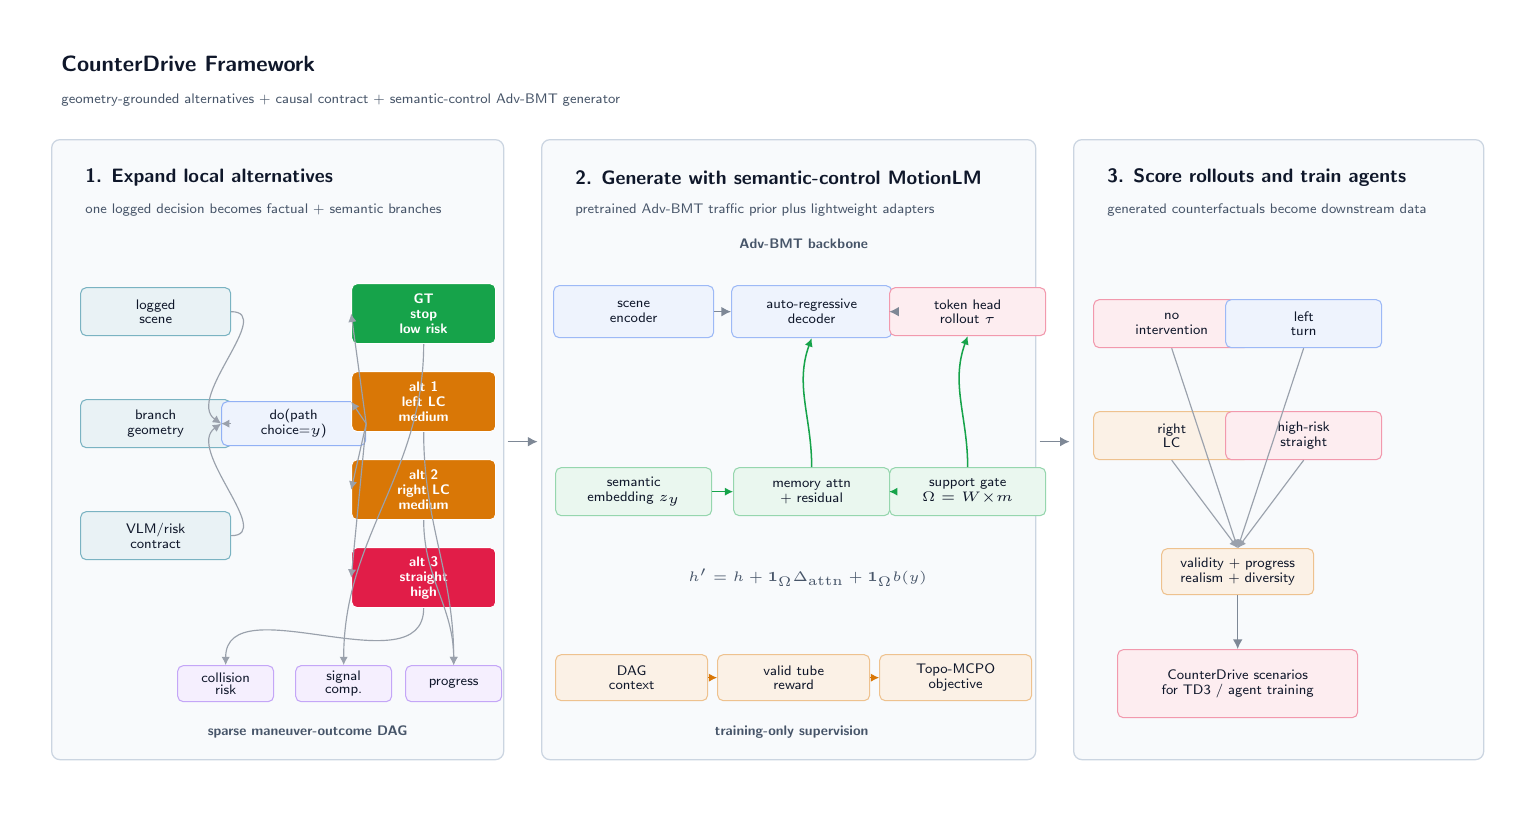
\begin{tikzpicture}[x=1in,y=1in]
  \fill[white] (0,0) rectangle (7.4,3.9);
  \node[anchor=west, text=ink, font=\bfseries\fontsize{8.4}{9.1}\selectfont] at (0.12,3.72)
    {CounterDrive Framework};
  \node[anchor=west, text=muted, font=\fontsize{5.1}{5.6}\selectfont] at (0.12,3.54)
    {geometry-grounded alternatives + causal contract + semantic-control Adv-BMT generator};

  % Three major panels.
  \draw[card] (0.12,0.24) rectangle (2.38,3.34);
  \draw[card] (2.57,0.24) rectangle (5.04,3.34);
  \draw[card] (5.23,0.24) rectangle (7.28,3.34);

  \draw[arrow] (2.40,1.83) -- (2.55,1.83);
  \draw[arrow] (5.06,1.83) -- (5.21,1.83);

  % Panel A: expanded DAG.
  \paneltitle{0.24}{3.15}{1. Expand local alternatives}
  \panelsubtitle{0.24}{2.99}{one logged decision becomes factual + semantic branches}

  \node[context] (scene) at (0.64,2.48) {logged\\scene};
  \node[context] (geom) at (0.64,1.92) {branch\\geometry};
  \node[context] (vlm) at (0.64,1.36) {VLM/risk\\contract};
  \node[dag, fill=blue!8, draw=blue!50] (choice) at (1.33,1.92) {do(path\\choice=$y$)};
  \draw[softarrow] (scene.east) to[out=0,in=145] (choice.west);
  \draw[softarrow] (geom.east) -- (choice.west);
  \draw[softarrow] (vlm.east) to[out=0,in=215] (choice.west);

  \riskbranch{gt}{1.98}{2.47}{GT\\stop}{green}{low risk}
  \riskbranch{altone}{1.98}{2.03}{alt 1\\left LC}{amber}{medium}
  \riskbranch{alttwo}{1.98}{1.59}{alt 2\\right LC}{amber}{medium}
  \riskbranch{altthree}{1.98}{1.15}{alt 3\\straight}{rose}{high}
  \foreach \b in {gt,altone,alttwo,altthree} {
    \draw[softarrow] (choice.east) -- (\b.west);
  }

  \node[outcomeSmall] (collide) at (0.99,0.62) {collision\\risk};
  \node[outcomeSmall] (comply) at (1.58,0.62) {signal\\comp.};
  \node[outcomeSmall] (progress) at (2.13,0.62) {progress};
  \draw[softarrow] (gt.south) to[out=-90,in=90] (comply.north);
  \draw[softarrow] (altone.south) to[out=-90,in=90] (progress.north);
  \draw[softarrow] (alttwo.south) to[out=-90,in=90] (progress.north);
  \draw[softarrow] (altthree.south) to[out=-90,in=90] (collide.north);
  \node[tinylabel] at (1.40,0.38) {sparse maneuver-outcome DAG};

  % Panel B: architecture.
  \paneltitle{2.69}{3.15}{2. Generate with semantic-control MotionLM}
  \panelsubtitle{2.69}{2.99}{pretrained Adv-BMT traffic prior plus lightweight adapters}

  \node[arch] (enc) at (3.03,2.48) {scene\\encoder};
  \node[arch] (dec) at (3.92,2.48) {auto-regressive\\decoder};
  \node[output] (head) at (4.70,2.48) {token head\\rollout $\tau$};
  \draw[arrow] (enc.east) -- (dec.west);
  \draw[arrow] (dec.east) -- (head.west);
  \node[tinylabel] at (3.88,2.82) {Adv-BMT backbone};

  \node[adapter] (sem) at (3.03,1.58) {semantic\\embedding $z_y$};
  \node[adapter] (adapt) at (3.92,1.58) {memory attn\\+ residual};
  \node[adapter] (gate) at (4.70,1.58) {support gate\\$\Omega=W{\times}m$};
  \draw[greenarrow] (sem.east) -- (adapt.west);
  \draw[greenarrow] (adapt.east) -- (gate.west);
  \draw[greenarrow] (adapt.north) to[out=90,in=250] (dec.south);
  \draw[greenarrow] (gate.north) to[out=90,in=250] (head.south);
  \node[tinylabel] at (3.90,1.15) {$h' = h + \mathbf{1}_{\Omega}\Delta_{\rm attn} + \mathbf{1}_{\Omega}b(y)$};

  \node[objective] (dagctx) at (3.02,0.65) {DAG\\context};
  \node[objective] (tube) at (3.83,0.65) {valid tube\\reward};
  \node[objective] (topo) at (4.64,0.65) {Topo-MCPO\\objective};
  \draw[orangearrow] (dagctx.east) -- (tube.west);
  \draw[orangearrow] (tube.east) -- (topo.west);
  \node[tinylabel] at (3.82,0.38) {training-only supervision};

  % Panel C: outputs and uses.
  \paneltitle{5.35}{3.15}{3. Score rollouts and train agents}
  \panelsubtitle{5.35}{2.99}{generated counterfactuals become downstream data}

  \node[output] (r1) at (5.72,2.42) {no\\intervention};
  \node[output, fill=blue!8, draw=blue!45] (r2) at (6.38,2.42) {left\\turn};
  \node[output, fill=amber!10, draw=amber!45] (r3) at (5.72,1.86) {right\\LC};
  \node[output, fill=rose!8, draw=rose!45] (r4) at (6.38,1.86) {high-risk\\straight};

  \node[objective] (score) at (6.05,1.18) {validity + progress\\realism + diversity};
  \draw[softarrow] (r1.south) -- (score.north);
  \draw[softarrow] (r2.south) -- (score.north);
  \draw[softarrow] (r3.south) -- (score.north);
  \draw[softarrow] (r4.south) -- (score.north);

  \node[output, minimum width=1.20in, minimum height=0.34in] (dataset) at (6.05,0.62)
    {CounterDrive scenarios\\for TD3 / agent training};
  \draw[arrow] (score.south) -- (dataset.north);

\end{tikzpicture}
\end{document}
